\documentclass[12pt]{article}
 
\usepackage[margin=1in]{geometry} 
\usepackage{amsmath,amsthm,amssymb}
\usepackage{graphicx}
\usepackage{float}
\newenvironment{statement}[2][Statement]{\begin{trivlist}
\item[\hskip \labelsep {\bfseries #1}\hskip \labelsep {\bfseries #2.}]}{\end{trivlist}}

\newtheorem{question}{Question}
\newenvironment{answer}{%
  \par\noindent\textbf{Answer:}\quad
}{%
  \hfill$\square$\par
}

\begin{document}
 
% --------------------------------------------------------------
%
%                         Start here
%
% --------------------------------------------------------------
 
\title{6.8300 Pset 4 Problem 1 writeup} % replace with the problem you are writing up
\author{Zhi Ren} % replace with your name
\maketitle

\section{Short-answer questions}
\begin{question}
Why are the MLP reconstructions so much less detailed than those produced by the SIREN?
\end{question}
\begin{answer}
The MLP reconstructions are less detailed than those produced by SIREN because the MLP is a piecewise linear function, which is not able to capture the high-frequency details in the image. In contrast, SIREN is a continuous function that can capture high-frequency details in the image. Additionally, Sine and Cosine functions form an orthogonal basis for reasonably smooth functions, thus SIREN enjoys certain transformation-invariance that MLP does not have, which also results in this difference in training outcomes. 
\end{answer}

\begin{question}
The image Laplacian produced by the MLP looks strange... what's happening here and why?
\end{question}
\begin{answer}
    The image Laplacian produced by the MLP looks strange because MLP has ReLU as its activation function, which is not twice differentiable (at zero). THe Laplacian operator acts on a function by taking its second derivatives, and the second derivatives of MLP are not smooth. Therefore, the naive implementation would not be able to produce high quality results for the Laplacian. 
\end{answer}


\section{Part III: Eeking out better performance!}
In this part, we experiment with 9 additional SIREN models and 9 additional MLP models with different hyperparameters. The hyperparameters that we choose to vary include the number of layers, and the number of hidden units. There are some additional hyperparameters that we could have varied, such as the learning rate, the optimizer, the activation function, etc. However, we choose to vary the number of layers and the number of hidden units because they are the most likely to have a significant impact on the performance of the model.

The hyperparameters that stay the same across all experiments include the following: the total training steps is kept at $2000$ and learning rate is kept at $1e-4$. The optimizer is Adam, and the activation function is ReLU for MLP and Sine for SIREN.

Below are the plots for losses and PSNRs for all the MLPs and SIRENs trained. 
\begin{figure}[h]
    \centering 
    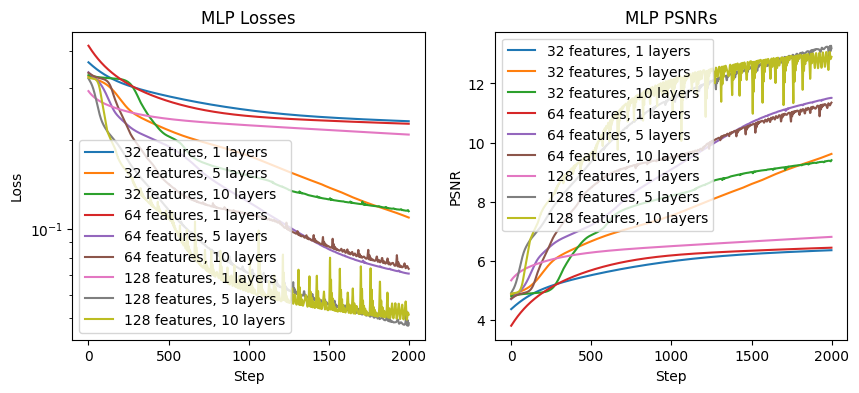
\includegraphics[width=1.0\textwidth]{LOSS_plot.png}
    \caption{MLPs}
\end{figure}
\begin{figure}[H]
    \centering 
    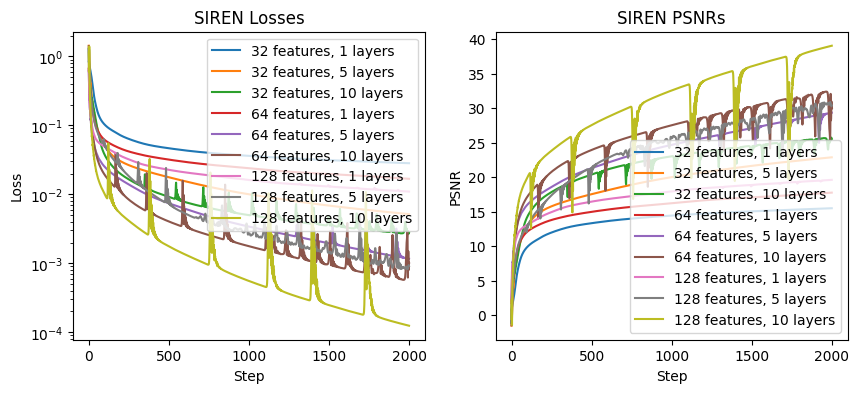
\includegraphics[width=1.0\textwidth]{PSNRs_plot.png}
    \caption{SIRENs}
\end{figure}

We see that the model that performs that best is SIREN with 128 features and 10 layers. We include the image reconstruction, gradient and Laplacian during the entire training process for this model below. 

\begin{figure}[h]
    \centering 
    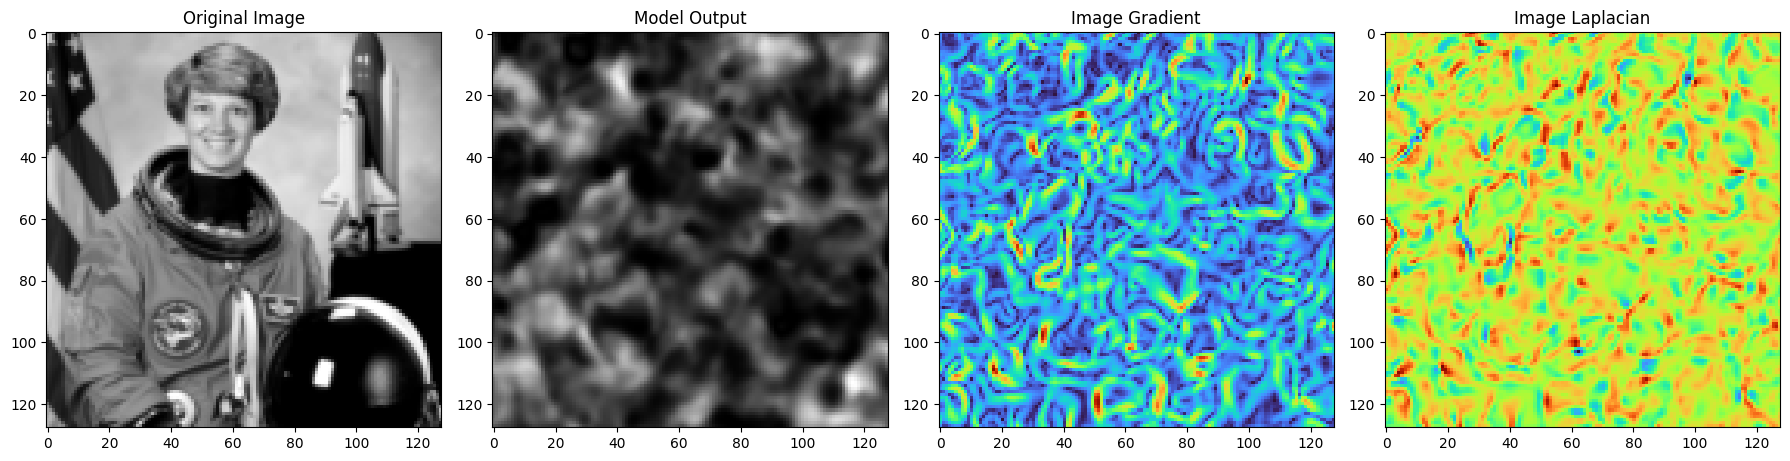
\includegraphics[width=1.0\textwidth]{training_plot1.png}
    \caption{Step200}
\end{figure}
\begin{figure}[h]
    \centering 
    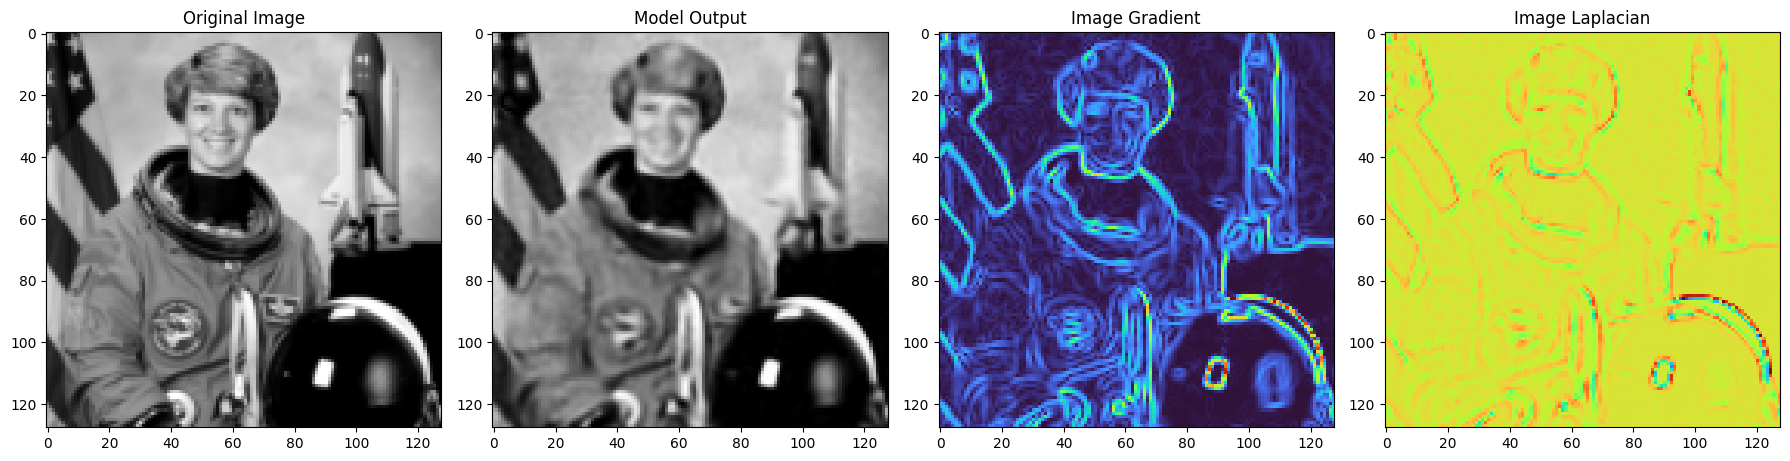
\includegraphics[width=1.0\textwidth]{training_plot2.png}
    \caption{Step400}
\end{figure}
\begin{figure}[h]
    \centering 
    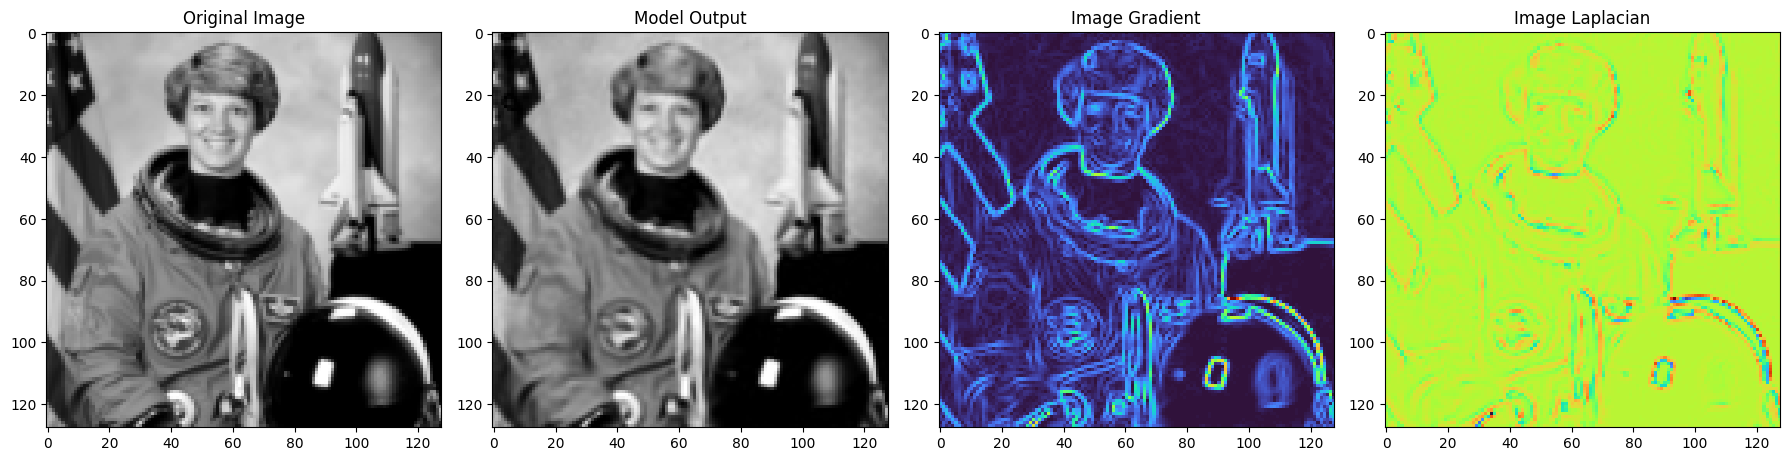
\includegraphics[width=1.0\textwidth]{training_plot3.png}
    \caption{Step600}
\end{figure}
\begin{figure}[h]
    \centering 
    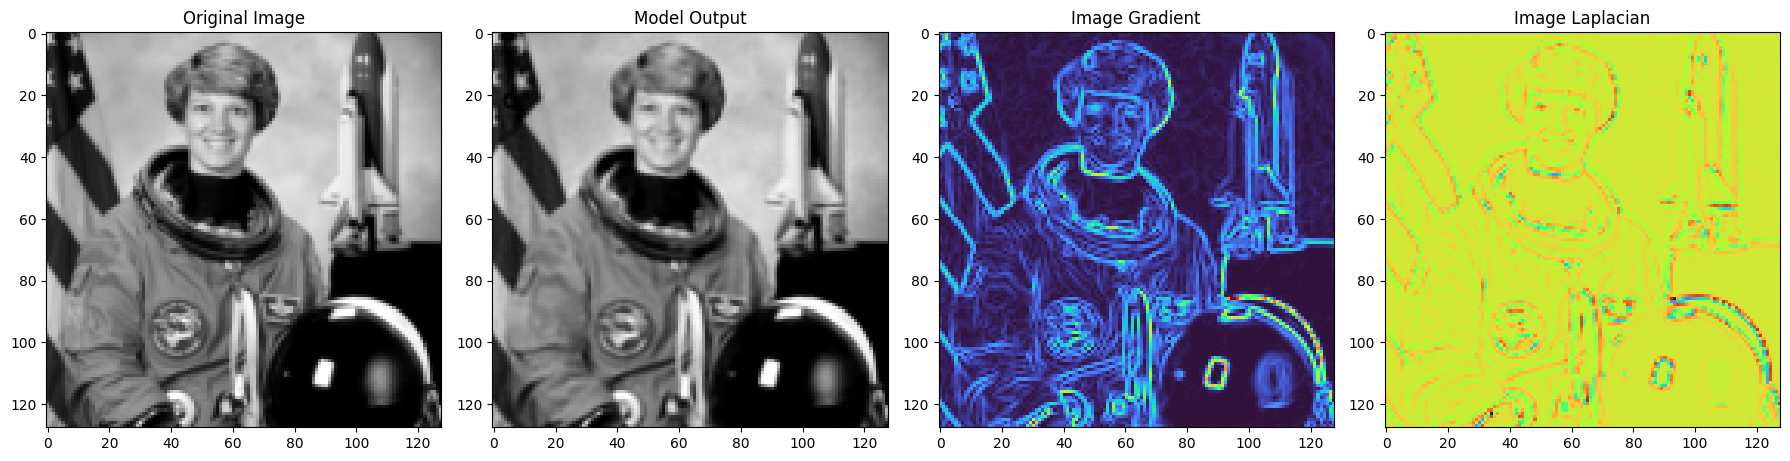
\includegraphics[width=1.0\textwidth]{training_plot4.png}
    \caption{Step800}
\end{figure}
\begin{figure}[h]
    \centering 
    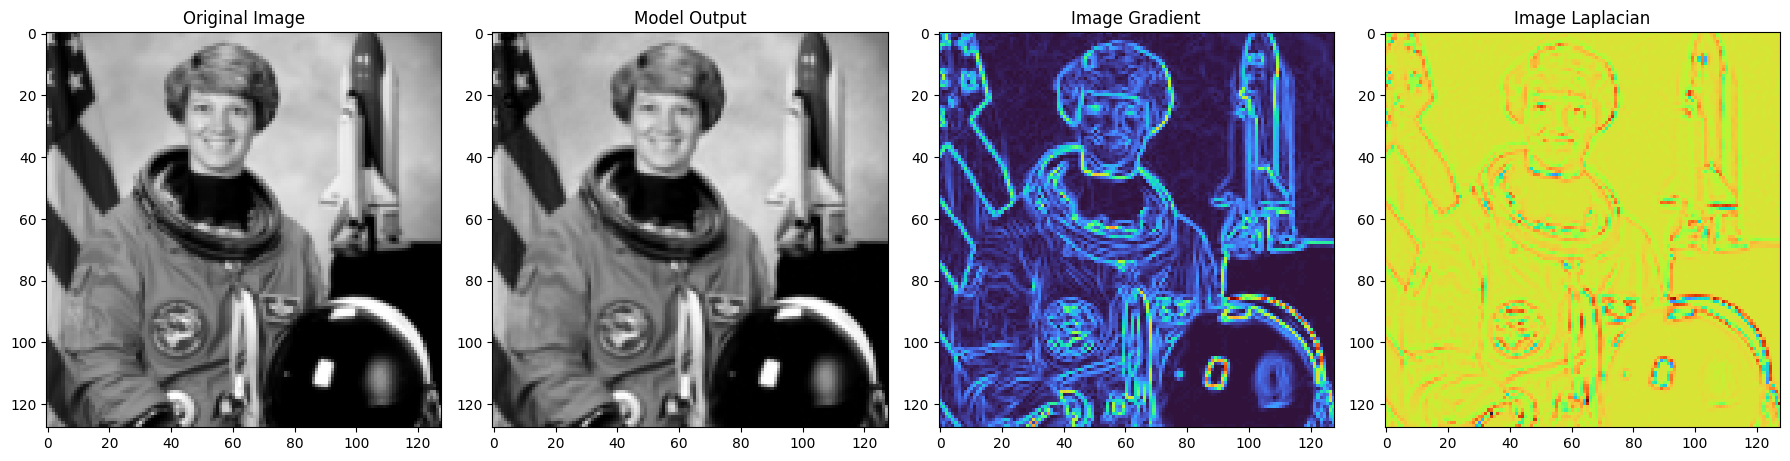
\includegraphics[width=1.0\textwidth]{training_plot5.png}
    \caption{Step1000}
\end{figure}
\begin{figure}[h]
    \centering 
    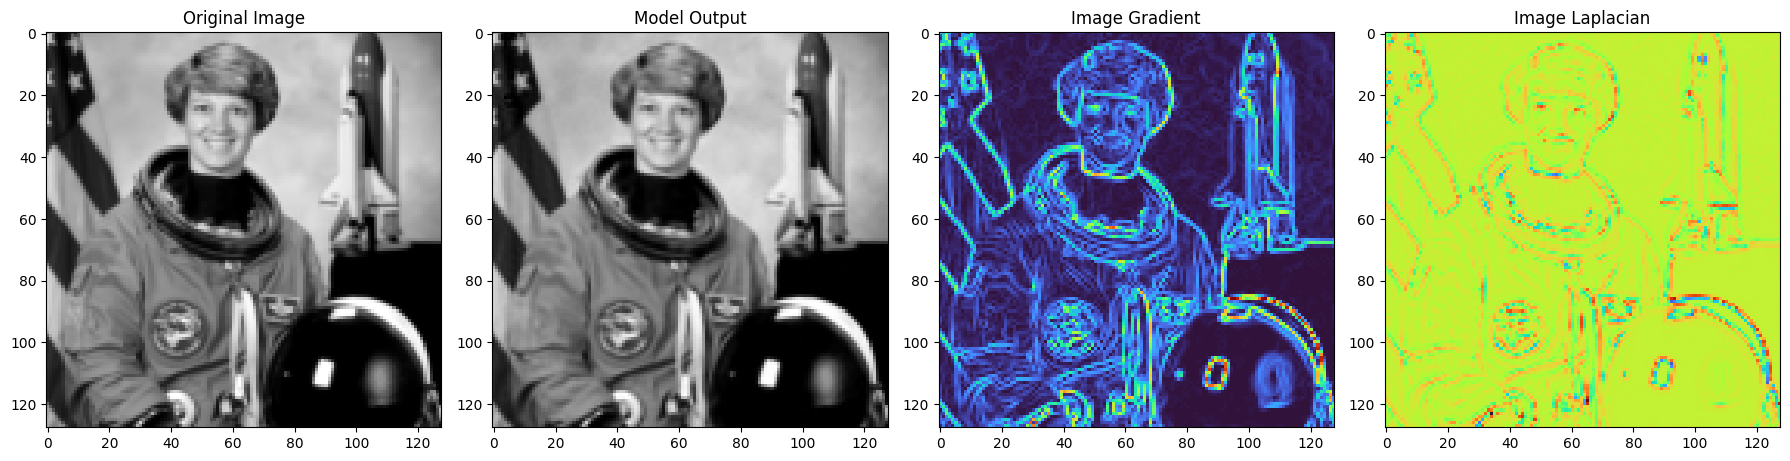
\includegraphics[width=1.0\textwidth]{training_plot6.png}
    \caption{Step1200}
\end{figure}
\begin{figure}[h]
    \centering 
    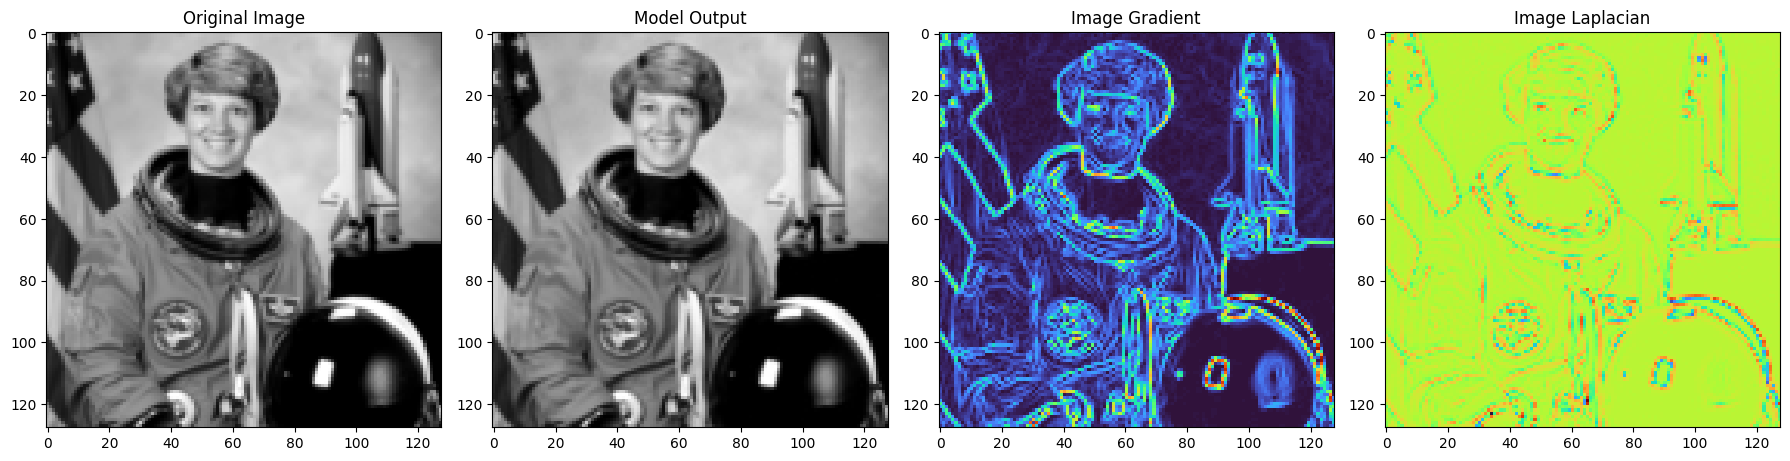
\includegraphics[width=1.0\textwidth]{training_plot7.png}
    \caption{Step1400}
\end{figure}
\begin{figure}[h]
    \centering 
    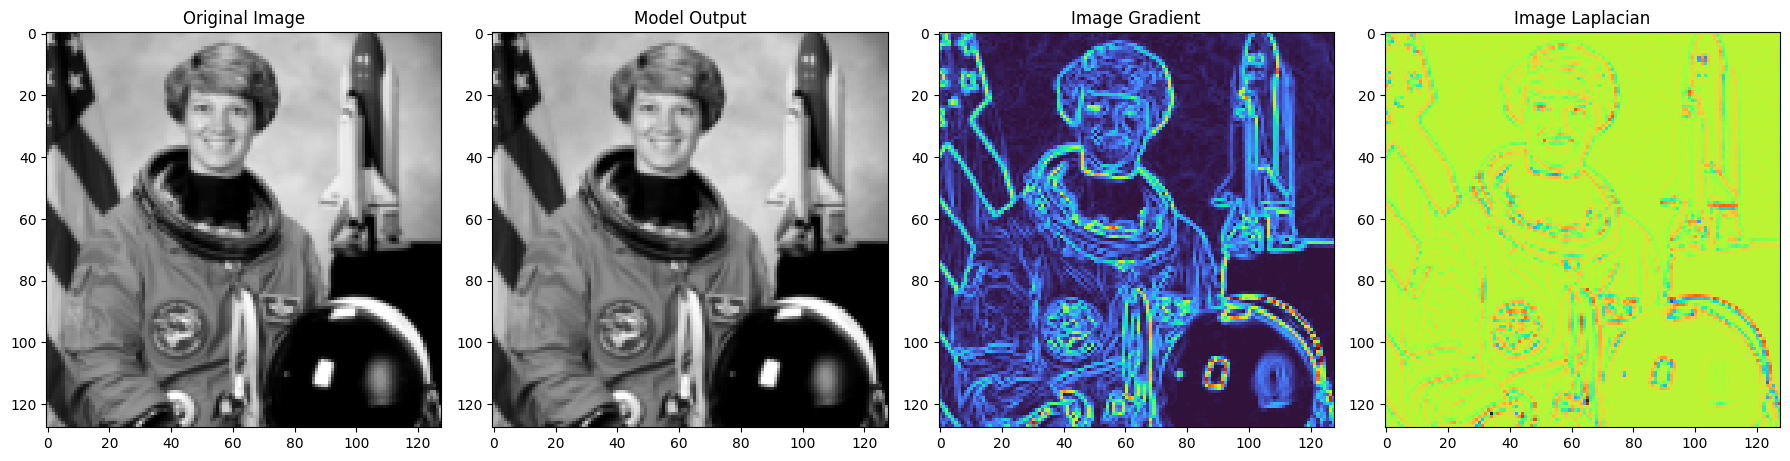
\includegraphics[width=1.0\textwidth]{training_plot8.png}
    \caption{Step1600}
\end{figure}
\begin{figure}[h]
    \centering 
    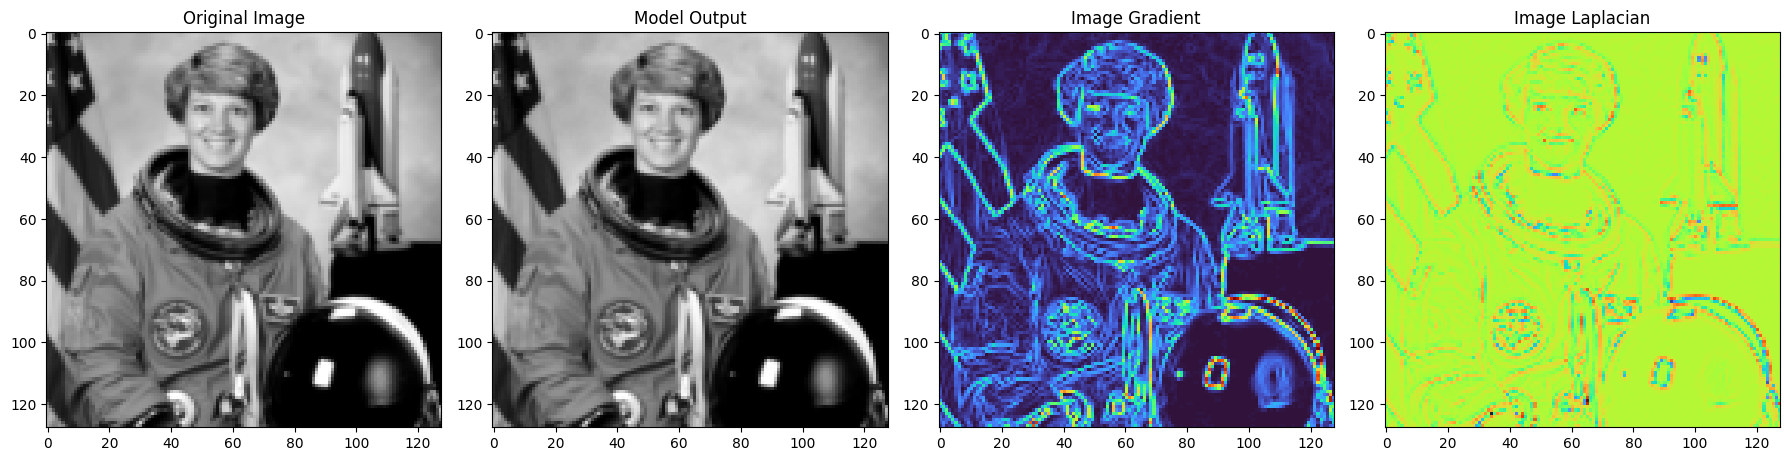
\includegraphics[width=1.0\textwidth]{training_plot9.png}
    \caption{Step1800}
\end{figure}
\begin{figure}[h]
    \centering 
    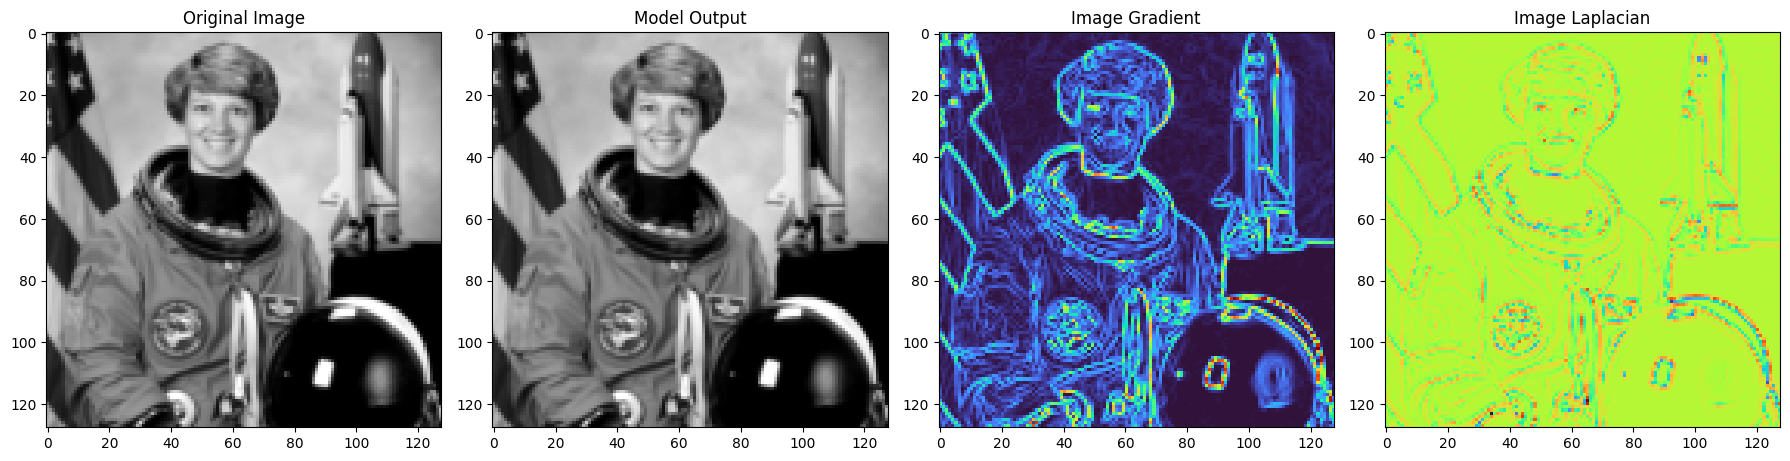
\includegraphics[width=1.0\textwidth]{training_plot10.png}
    \caption{Step2000}
\end{figure}














\end{document}